% -*- mode: noweb; noweb-default-code-mode: R-mode; -*-
\documentclass[11pt]{article}
%% Set my margins
\setlength{\oddsidemargin}{0.0truein}
\setlength{\evensidemargin}{0.0truein}
\setlength{\textwidth}{6.5truein}
\setlength{\topmargin}{0.0truein}
\setlength{\textheight}{9.0truein}
\setlength{\headsep}{0.0truein}
\setlength{\headheight}{0.0truein}
\setlength{\topskip}{0pt}
%% End of margins

%%\pagestyle{myheadings}
%%\markboth{$Date$\hfil$Revision$}{\thepage}

\usepackage[pdftex,
bookmarks,
bookmarksopen,
pdfauthor={Zequn Sun, Wei Wei and Dongjun Chung},
pdftitle={PICS Vignette}]
{hyperref}

% \usepackage{fullpage}
% \usepackage{pdflscape}

\title{An Introduction to the `\texttt{PICS}' Package, Version 1.0}
\author{ Zequn Sun,Wei Wei and Dongjun Chung\\
Department of Public Health Sciences, Medical University of South Carolina (MUSC),\\
  Charleston, SC, 29425.}


\date{\today}



\usepackage{Sweave}
\begin{document}
\Sconcordance{concordance:PICS-example.tex:C:/Users/dchung/Google Drive/USB/research - 20. cancer subtype identification/1. pathway_index/software/PICS/vignettes/PICS-example.Rnw:%
1 36 1 1 0 23 1 1 4 1 2 4 0 1 2 19 1 1 2 1 0 1 1 10 0 1 1 5 0 1 1 5 0 1 %
1 12 0 1 2 4 1 1 2 4 0 1 2 15 1 1 2 4 0 1 2 16 1 1 2 1 0 1 1 21 0 1 2 %
15 1 1 2 4 0 1 2 3 1 1 -5 1 9 8 1 1 2 1 0 1 1 18 0 1 2 7 1 1 2 26 0 2 2 %
4 0 1 2 5 1 1 -7 1 11 10 1 1 2 4 0 1 2 3 1 1 -5 1 9 16 1}

%\VignetteIndexEntry{PICS}
%\VignetteKeywords{PICS}
%\VignettePackage{PICS}
%\VignetteEncoding{UTF-8}
\maketitle

\section{Overview}

This vignette provides basic information about the
\texttt{PICS}`\cite{PICS}' package. PICS stands for ``Pathway-guided Identification of Cancer Subtypes''.
The \texttt{PICS} methodology for Pathway-Guided Identification of Cancer Subtypes is developed in \texttt{PICS}. The proposed approach improves identification of molecularly-defined subgroups of cancer patients by utilizing information from pathway databases in the following four aspects.

(1) integration of genomic data at the pathway-level improves robustness and stability in identification of cancer subgroups and driver molecular features; and

(2) summarizing multiple genes and genomic platforms at the pathway-level can potentially improve statistical power to identify important driver pathways because moderate signals in multiple genes can be aggregated; and

(3) in \texttt{PICS}, we consider this ``operation'' or ``interaction'' between pathways, instead assuming that each pathway operates independently during the cancer progression, which may be unrealistic; and

(4) \texttt{PICS} allows simultaneous inference in multiple biological layers (pathway clusters, pathways, and genes) within a statistically rigorous and unified framework without any additional laborious downstream analysis.

The package can be loaded with the command:


\begin{Schunk}
\begin{Sinput}
R> library("PICS")
\end{Sinput}
\end{Schunk}

\section{Input Data}

The package requires that the response consist of 4 components:
(1) z-scores in the form of a either data frame or matrix; and
(2) time and status variable for Cox model of survival analysis in the form of vectors; and
(3) pathway information is in the form of a list where gene names are included in pathway lists respectively.

The Cancer Genome Atlas (TCGA) is an example application for the `\texttt{PICS}' package.
The TCGA data was downloaded from the cBio Portal (http://www.cbioportal.org/) using the R package `\texttt{cgdsr}', and we used z scores for the mRNA expression data.

All the mRNA expression measures were centered and scaled to have unit variance according to standard practice. Only genes annotated in the KEGG database and that appeared in both datasets were considered for analysis. In the current stage, we focused only on gene expression measurements and aim at incorporating other data types into our model in the future.

The `\texttt{TCGA}' is a list object with four elements, including the `\texttt{geneexpr}' data frame of z scores for the mRNA expression, the `\texttt{t}' vector of the survival time, the `\texttt{d}' vector of the survival status indicator, and the `\texttt{pathList}' list of the pathway information. The `\texttt{pathList}' has four elements, each of which contains names of genes belonging to each pathway. Z scores for the mRNA expression data of 389 genes are provided for 50 cancer patients, along with survival times and survival statuses.

This dataset can be loaded as follows:

\begin{Schunk}
\begin{Sinput}
R> data(TCGA)
R> TCGA$geneexpr[1:5,1:5]
\end{Sinput}
\begin{Soutput}
        ACLY        ACO1       ACO2         CS       DLAT
1 -2.2410125 -0.48445531 -1.6346455  0.1378804 -3.5310321
2 -2.1301362  0.82116427 -0.9533701  0.6213512  0.6689948
3 -2.9122727 -0.08790649 -1.0975096 -0.2454025 -0.9433900
4 -1.1721514 -0.24249825 -0.7212639  0.1842386 -0.6188785
5  0.5383438  0.98012739 -0.7396043 -0.0699680  1.9573767
\end{Soutput}
\begin{Sinput}
R> TCGA$t[1:5]
\end{Sinput}
\begin{Soutput}
[1] 43.89 40.97 49.12  2.00 46.59
\end{Soutput}
\begin{Sinput}
R> TCGA$d[1:5]
\end{Sinput}
\begin{Soutput}
[1] 1 1 0 1 0
\end{Soutput}
\begin{Sinput}
R> TCGA$pathList[1]
\end{Sinput}
\begin{Soutput}
$KEGG_CITRATE_CYCLE_TCA_CYCLE
 [1] "IDH3B"     "DLST"      "PCK2"      "CS"        "PDHB"      "PCK1"     
 [7] "PDHA1"     "LOC642502" "PDHA2"     "LOC283398" "FH"        "SDHD"     
[13] "OGDH"      "SDHB"      "IDH3A"     "SDHC"      "IDH2"      "IDH1"     
[19] "ACO1"      "ACLY"      "MDH2"      "DLD"       "MDH1"      "DLAT"     
[25] "OGDHL"     "PC"        "SDHA"      "SUCLG1"    "SUCLA2"    "SUCLG2"   
[31] "IDH3G"     "ACO2"     
\end{Soutput}
\end{Schunk}

\section{Pre-filtering}

We expected that only a parsimonious set of genes would be related to patient survival, i.e., the sparsity assumption. To eliminate the most unlikely predictors, we first conducted a supervised pre-filtering by fitting a Cox regression model of each mRNA expression measure on patient survival in the TCGA dataset. Only the gene expressions associated with patient survival at p-values smaller than a pre-specified cut-off were included in the subsequent analysis. Here we chose p = 0.5 as the default cut-off point.

\begin{Schunk}
\begin{Sinput}
R> train.list=prefilter(data=TCGA$geneexpr, time=TCGA$t, status=TCGA$d, plist=TCGA$pathList)
R> train.list
\end{Sinput}
\begin{Soutput}
Summary: Pre-filtering results (class: Prefiltered)
--------------------------------------------------
Number of genes before prefiltering: 389
Number of genes after prefiltering: 213
--------------------------------------------------
\end{Soutput}
\end{Schunk}

\section{Gene Selection}
This section is about Gene-level Analysis using a SPLS\cite{SPLS} Cox regression. In order to select key genes associated with patient survivals and effectively summarize them by taking into account correlation among them, we fit a sparse partial least squares (SPLS) Cox regression model of patient survivals on gene expression measurements for each pathway.

\texttt{PICS} utilizes extention of SPLS Cox regression so that it can handle survival outcomes, where there are two main tuning parameters: `\texttt{eta}' represents
the sparsity tuning parameter and `\texttt{K}'
is the number of hidden (latent) components. Parameters can be chosen by ($v$-fold)
cross-validation using the
function `\texttt{selectGene}'.  The user specifies the range for these parameters and
the cross-validation procedure
searches within these ranges. `\texttt{eta}' should have a value between 0 and 1. `\texttt{K}'
is integer valued and can range between
1 and $ min \left\{ p, (v-1) n / v \right\} $, where $p$ is the number of predictors and $n$ is the sample size. For example, if 10-fold cross-validation is used (default), `\texttt{K}' should be smaller than $ min \left\{ p, 0.9 n \right\} $. For the TCGA data, we set fold as 5, `\texttt{K}' as 5, and search for `\texttt{eta}' among 0.1, 0.5 and 0.9
with the following command:


\begin{Schunk}
\begin{Sinput}
R> gene.results=selectGene( train.list, fold=5, K=5, etas=c(0.1,0.5,0.9) )
\end{Sinput}
\end{Schunk}
\begin{Schunk}
\begin{Sinput}
R> gene.results
\end{Sinput}
\begin{Soutput}
Summary: Gene-level analysis results (class: FitGene)
--------------------------------------------------
Number of prefiltered genes: 213
Number of selected genes: 200
--------------------------------------------------
\end{Soutput}
\end{Schunk}

The function `\texttt{selectGene}' returns the following output:

(1) Score: the latent variables summarizing the gene expression data in each pathway, scores are linear combinations of the original gene expression data.

(2) geneSelected: cancer related genes selected by our approach.

(3) fit: including list of 'coef' and 'direction'. 'coef' is the list of the SPLS regression coefficients of cancer related genes; 'direction' is the list of the direction vectors \texttt{W} for constructing scores, where $score = X \times W$, and \texttt{X} is the original gene expression data.

(4) dataPrefiltered: output list of prefilter step.

(5) inputdata: input list of prefilter step.



\section{Pathway Selection}

Next, in order to identify a parsimonious set of pathways associated with patient survivals, we fit a LASSO-penalized\cite{LASSO} Cox regression on latent components derived from all the pathways.
First, the latent components generated from the SPLS step preserve pathway structure and also reflect correlation among genes and their association with survival outcomes. Second, this approach can potentially improve the stability of estimation in the subsequent analysis.
\begin{Schunk}
\begin{Sinput}
R> path.results=selectPath( gene.results )
R> path.results
\end{Sinput}
\begin{Soutput}
Summary: Pathway-level analysis results (class: FitPath)
--------------------------------------------------
Number of all pathways: 4
Number of selected pathways: 4

List of selected pathways:
	KEGG_CITRATE_CYCLE_TCA_CYCLE:
	KEGG_MAPK_SIGNALING_PATHWAY:
	KEGG_TGF_BETA_SIGNALING_PATHWAY:
	KEGG_THYROID_CANCER:
--------------------------------------------------
\end{Soutput}
\end{Schunk}
The function `\texttt{selectPath}' returns the following output:

(1) pathAll: pathways that were left from pre-filtering step.

(2) pathSelected: cancer related pathways selected by our approach.

(3) coef: data frame of LASSO regression coefficients of cancer related pathways.

(4) fitGene: output list of selectGene step.


\section{Pathway Effect Plot}
In the LASSO step, we could identify the pathways associated with patient survivals using the latent components generated from the SPLS step.

Specifically, a pathway was selected if at least one of its latent components had non-zero LASSO coefficient estimate. Figure 1 shows the hazard ratio (HR) associated with each latent component in selected pathways.

Based on the TCGA data, pathways with the largest effect on survival ($HR \geq 1.15$) are \texttt{CITRATE\_CYCLE\_TCA\_CYCLE} and \texttt{MARK\_SIGNALING} pathways.

\begin{Schunk}
\begin{Sinput}
R> plot(path.results, type="HR")
\end{Sinput}
\end{Schunk}


\begin{figure}[tbh]
\begin{center}
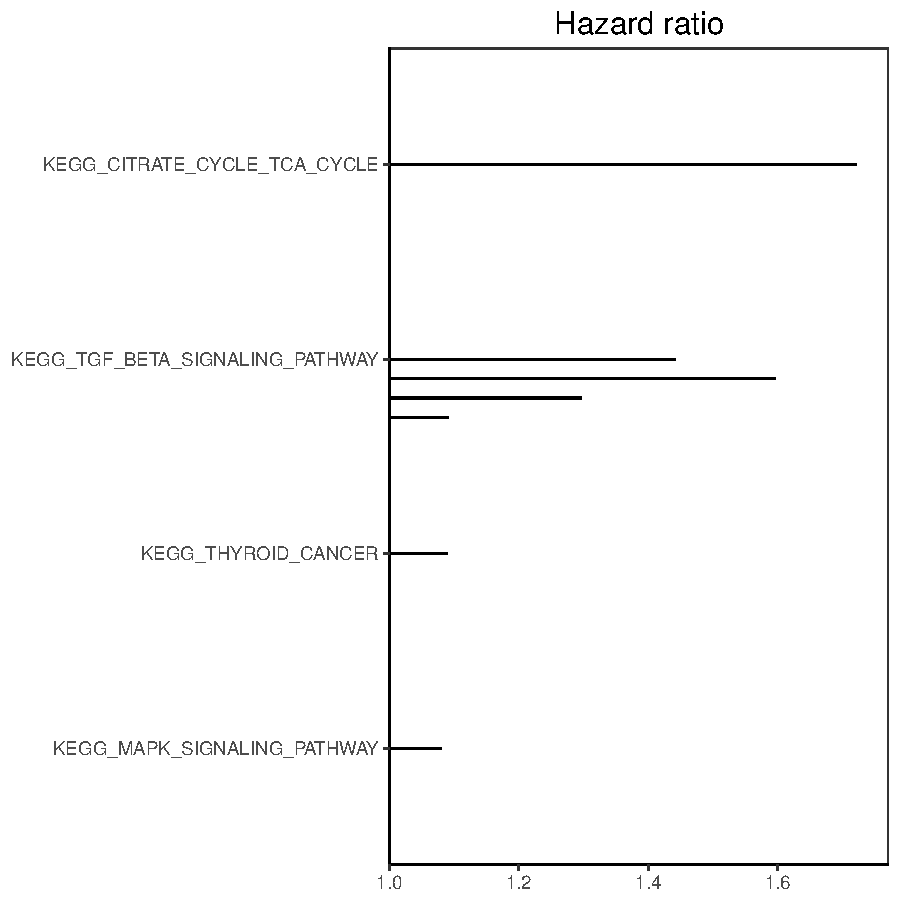
\includegraphics{PICS-example-plot1}
\caption{Hazard ratio (HR) associated with each latent component in selected pathways}
\end{center}
\end{figure}



\section{Prediction}
Survival predictions were made based on model parameters estimated from the TCGA data.

\begin{Schunk}
\begin{Sinput}
R> predicted=predict(path.results)
R> predicted[1:3]
\end{Sinput}
\begin{Soutput}
$risk.index
 [1] 3 4 0 4 1 4 4 0 0 1 4 1 2 3 3 3 0 1 0 3 2 0 1 1 2 2 3 0 1 0 2 0 1 0 0 0 1 0
[39] 4 3 2 4 4 4 4 4 3 4 3 3

$riskcat
 [1] "high" "high" "low"  "high" "med"  "high" "high" "low"  "low"  "med" 
[11] "high" "med"  "med"  "high" "high" "high" "low"  "med"  "low"  "high"
[21] "med"  "low"  "med"  "med"  "med"  "med"  "high" "low"  "med"  "low" 
[31] "med"  "low"  "med"  "low"  "low"  "low"  "med"  "low"  "high" "high"
[41] "med"  "high" "high" "high" "high" "high" "high" "high" "high" "high"

$cuts
[1] 0.25 3.00
\end{Soutput}
\end{Schunk}

\section{Survival Curve}
The predictive performance of \texttt{PICS} method was presented by Kaplan-Meier curves.
`\texttt{survivalCurve}' returns Kaplan-Meier curves of predicted patient subgroups based on the \texttt{PICS} approach.

\begin{Schunk}
\begin{Sinput}
R> summary( coxph(Surv(predicted$time, predicted$status) ~ predicted$riskcat) )
\end{Sinput}
\begin{Soutput}
Call:
coxph(formula = Surv(predicted$time, predicted$status) ~ predicted$riskcat)

  n= 50, number of events= 35 

                         coef exp(coef) se(coef)      z Pr(>|z|)    
predicted$riskcatlow -3.97566   0.01877  1.05057 -3.784 0.000154 ***
predicted$riskcatmed -1.18684   0.30518  0.39768 -2.984 0.002841 ** 
---
Signif. codes:  0 '***' 0.001 '**' 0.01 '*' 0.05 '.' 0.1 ' ' 1

                     exp(coef) exp(-coef) lower .95 upper .95
predicted$riskcatlow   0.01877     53.285  0.002394    0.1471
predicted$riskcatmed   0.30518      3.277  0.139977    0.6654

Concordance= 0.769  (se = 0.053 )
Rsquare= 0.533   (max possible= 0.987 )
Likelihood ratio test= 38.07  on 2 df,   p=5.402e-09
Wald test            = 19.64  on 2 df,   p=5.443e-05
Score (logrank) test = 34.55  on 2 df,   p=3.152e-08
\end{Soutput}
\end{Schunk}

\begin{Schunk}
\begin{Sinput}
R> plot(path.results,type="KM")
\end{Sinput}
\end{Schunk}

Figure 2 shows the Kaplan-Meier curves of predicted patient subgroups based on the \texttt{PICS} approach. The \texttt{PICS} approach could distinguish the high risk group from the medium risk (log rank test, p=0.0075) and low risk (log rank test, p=0.00005) groups.
% but could not distinguish the medium risk group from the low risk group (log rank test, p=0.850).

\begin{figure}[tbh]
\begin{center}
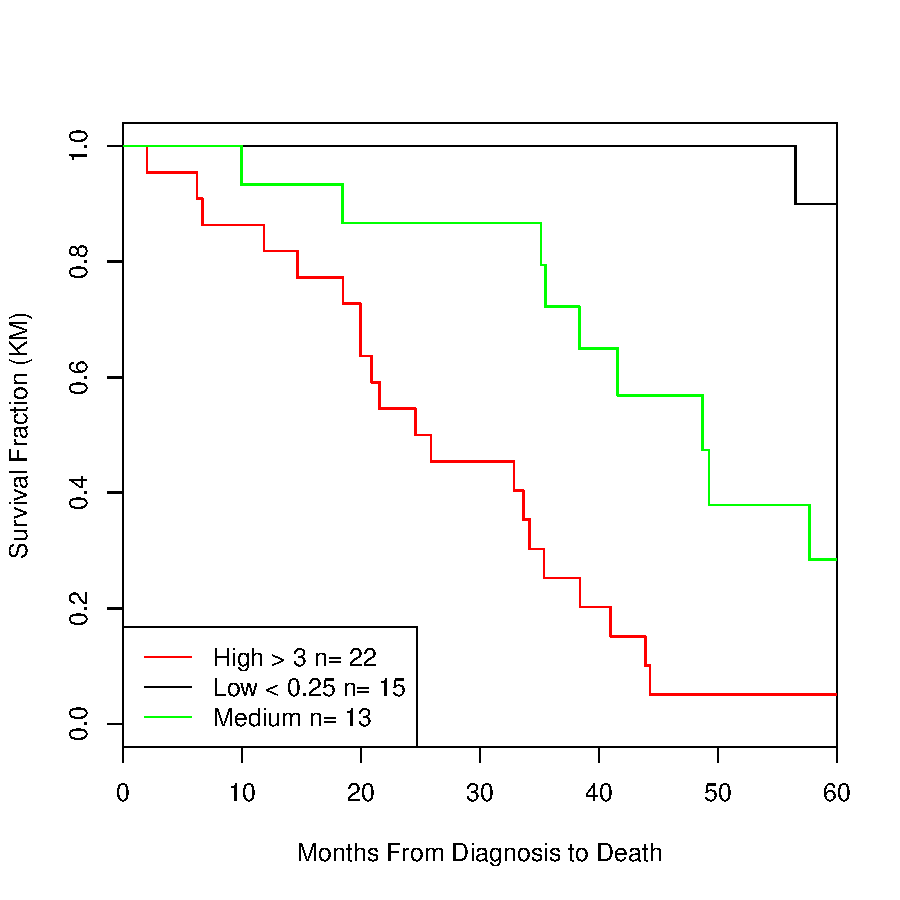
\includegraphics{PICS-example-plot}
\caption{The observed survival curves for patient subgroups identified by the \texttt{PICS}}
\end{center}
\end{figure}

\section{Survival ROC}

The predictive performance of \texttt{PICS} method was further evaluated based on area under the time dependent receiver operating curve (ROC).
`\texttt{survivalROC}' returns a ROC for survival plot.
\begin{Schunk}
\begin{Sinput}
R> plot(path.results,type="ROC")
\end{Sinput}
\end{Schunk}


\begin{figure}[tbh]
\begin{center}
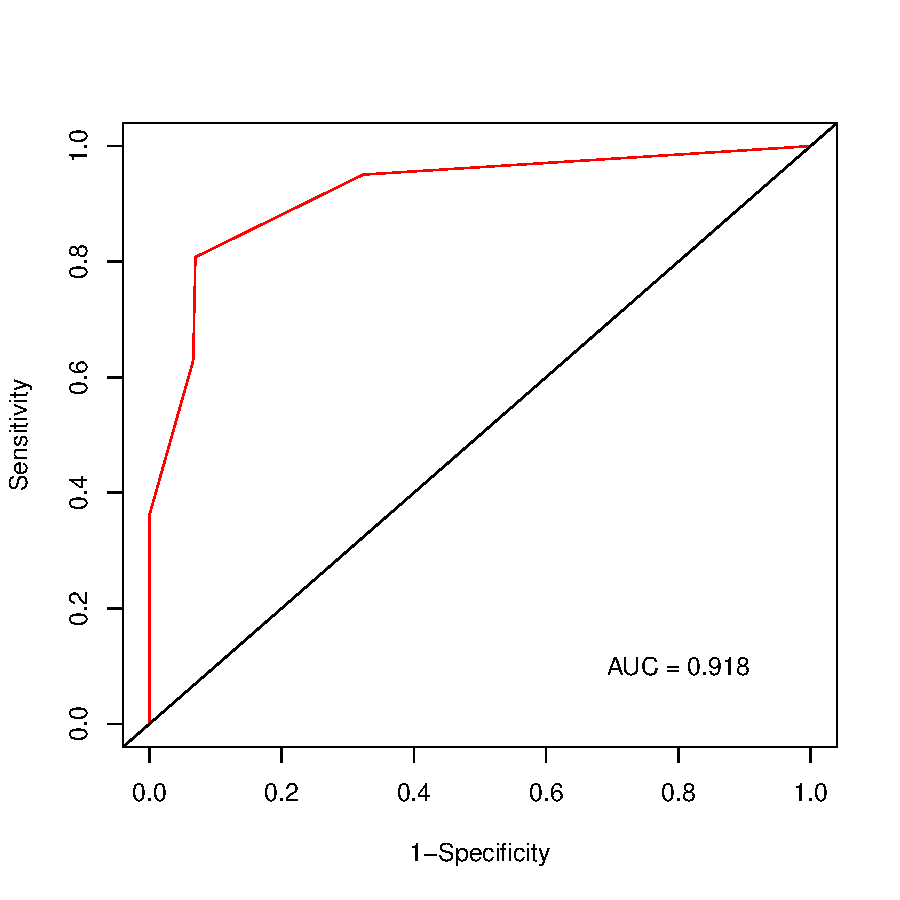
\includegraphics{PICS-example-plot3}
\caption{Time dependent Receiver Operating Curves}
\end{center}
\end{figure}

Figure 3 shows the ROC curves for survival and demonstrates an advantage of the \texttt{PICS} approach. For the TCGA data, the area under curve (AUC) associated with the \texttt{PICS} approach was 0.918.


\begin{thebibliography}{99}
\bibitem{PICS} Wei Wei, Zequn Sun, Willian da Silveira, Zhenning Yu, Andrew Lawson, Gary Hardiman, Linda Kelemen, Dongjun Chung (2017), ``PICS: Pathway-guided identification of cancer subtypes''. (submitted).
\bibitem{TCGA} Cancer Genome Atlas Research Network (2011), ''Integrated genomic analyses of ovarian carcinoma'', Nature, 474(7353):609-615.
\bibitem{SPLS} Chun, H. and Kele\c{s}, S. (2007) ``Sparse partial least squares
  for simultaneous dimension reduction and variable selection'',
(\url{http://www.stat.wisc.edu/~keles/Papers/SPLS_Nov07.pdf}).
\bibitem{LASSO} Tibshirani, R. (1996), ''Regression Shrinkage and Selection via the Lasso'', Journal of the Royal Statistical Society (Series B), 58, 267-288.
\end{thebibliography}

\end{document}
